\section{\textbf{Methods}}

% how did I solve the problem?

% FUNDAMENTALLY, doing synthesis on the shipping, with a set of simple rules to validate observations.
% shipping as sensor network -- a synthesis.

\subsection{Volunteered vessel information}

%"In short, changing technology and economics are moving map production from a system of unified central production to a local patchwork, and the old radial system of dissemination is being replaced with a complex network."
% -- Goodchild cartography paper, old and captures the change in production that is ongoing.

%\citep{elwood2011researching} includes reference to these same layers, capturing data on 'core' data layers independently. Covers much of what Goodchild has discussed in terms of issues with VGI and its current 'cutting edge'
Historically, ship data was collected both by governments for internal use, and by private corporations with the intent to sell. As elsewhere in the production of geographic facts, a shift is underway which moves the emphasis away from top-down primary data collection, to relying on observations from a multitude of sources \citep{goodchild2007citizens,elwood2011researching}. This new information has the potential to fundamentally change our use of the ocean.

% Using two kinds of volunteered ship data - needs to be handled in special ways:
% describe VOSclim data:
Ship captains have long taken climate observations alongside known locations \citep{brohan2009marine}.  Building on this history, the Voluntary Observing Ship (VOS, \citealp{VOSOverview}) program collected a dataset spanning over 20 years and covering 10\textendash20\% of commercial traffic within each year. Ass the intention was to collect open-ocean climate observations, many of the records lack ship attribute information. % XXX making trajectory reconstruction difficult. 
The data is contained within the greater International Comprehensive Ocean-Atmosphere Data Set (ICOADS, \citealp{woodruff2010icoads}), and though the data is both spatially- and statistically- biased \citep{Wang2007}, it serves as a useful training dataset on ship movements in the open ocean. Here, I use VOS records from 2003--2011, supplemented with opportunistic observations collected by the vessel tracking site SailWX \citep{SAILWX}. On the vessels that do report both attributes and locations, this information is captured at regular intervals, providing difficult to find open ocean observations.
% XXX: what other data does SailWX also include? YOTREPS? what else?

% describe AIS data
The Automatic Identification System (AIS) \citep{no20041028,Tetreault2002} was developed to improve maritime safety and prevent collisions, by providing mariners local situational awareness (Figure \ref{fig:ais-overview}). By locating the ships via global positioning satellite (GPS) fix, and broadcasting the location alongside other attributes (Table \ref{table:ais-broadcast-attributes}) regularly via VHF transceiver, mariners gain real-time local traffic, invaluable in inclement weather or rescue operations \citep{Itu-r2010}.  The International Maritime Organization (IMO) mandates that all ships $\geq\negthickspace 150$ gross tonnage (GT) or ships bearing paid passengers carry AIS units \citep{solas}, which has lead to approximately 200,000 ships being outfitted with AIS equipment, including all licensed tankers, cargo ships and passenger vessels. Because the intent was to improve maritime safety, the system uses well-understood VHF radios, broadcasting to about 40km between ships. Since the system's implementation, land-based users, including ports, maritime professionals and amateurs, have set up VHF antennae, providing low-cost local ship traffic data at a range of up to 100km. Numerous sites now provide real-time feeds, such as MarineTraffic \citep{MarineTraffic} and SailWX, aggregating the records from many land-based antennae (and more recently, satellite feeds) and displaying them over both web maps and via Google Earth. These sites constantly augment their networks by providing in-depth data to those willing to set up AIS receiving stations in geographic areas not yet covered.

\begin{figure}[htbp]
  \centering
  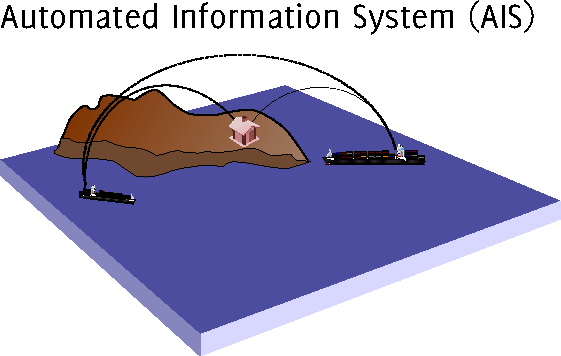
\includegraphics[width=100mm]{images/towers/drawing.pdf}
  \caption{Automated Information System diagram. Ships communicate to one another via VHF broadcast. The same signals can be captured and stored by land- and satellite- based observers.}
  \label{fig:ais-overview}
\end{figure}

\subsection{Data Collection}

For this study, fifteen months of AIS data were collected, from November 2010--December 2011, aggregating records from three major online AIS providers: FleetMon, VesselTracker, and MarineTraffic. All three share Keyhole Markup Language (KML, \citeauthor{KML}) files, intended for Google Earth. Examining data availability (Figure \ref{fig:ais-coverage}) showed these providers had considerably different coverage. At ten minute intervals over the study period, I automated downloading these KML files of real-time ship traffic from each of the providers. I then parsed the files to extract each observation within the dataset, wrote a library to normalize differences between the providers, and inserted the results into a spatial database, (PostGIS, \citeauthor{ramsey2005postgis}), an extension providing support for OGC simple features \citep{OGCSimple} on top of the PostgreSQL \citep{postgresql} object-relational database engine). Over the study period, this provided 2.37 billion observations which all include ship location and time, but frequently include additional attributes (Table \ref{table:ais-broadcast-attributes}).  The VOS/SailWX dataset, consisting of 92.4 million records covering Feburary 1991--September 2011, was provided in a MySQL database dump, which was converted and imported into PostgreSQL. 

Augmenting these ship observations, ancillary data was identified to provide validation against the raw observations, which is described below.

\subsubsection{Vessel attribute data}
Vessel data, tabular lists of ships alongside attributes, was collected from both authoritative and crowd-sourced media (Table \ref{table:ships-data-sources}) from a variety of sources, useful in validating the attributes provided in both VOS and AIS observations. Sources include:
\begin{enumerate}
  \item Within the United States, the Federal Communications Commission (FCC) regulates the airwaves. In order to track and manage radio licenses, the FCC has developed the Consolidated Database System (CDBS), which includes information on all vessels with registered radios within the US. 
  \item The International Telecommunications Union (ITU) created the Maritime mobile Access and Retrieval System (MARS) database to provide the maritime community with the most up-to-date data for registered vessels. Thanks to their role as a regulating body, participant states are required to provide up-to-date information. This database is particularly useful as it includes details not available through other public means, such as the vessel owner, and passenger capacity.
  \item DigitalSeas provided volunteered vessel attribute information, collected primarily through corrected AIS observations, but has since gone off-line.
  \item VesselTracker includes ship tracking, reporting and vessel records, alongside real-time AIS position data. Both their vessel data, and their AIS observations were recorded in this study. The dataset shows particular strength in European waters. Vesseltracker has also developed a ship routing network, but doesn't provide public access to this resource.
\end{enumerate}

\subsubsection{Land-sea mask}
\label{sec:land-sea-mask}
  A high resolution land-sea mask, derived from the Shuttle Radar Topography Mission (SRTM) Water Body Data (SWBD, \citealp{slater2006srtm}), classifies the world into either land or sea at three arcsecond resolution (\textasciitilde{}90m) for much of the world (56$^\circ$ S to 60$^\circ$ N). It was a by-product of the SRTM digital terrain project \citep{rabus2003shuttle}, and has the advantage that the data was collected over a very short period of time, increasing self-consistency.

For the areas beyond that covered by SRTM, the Global Self-consistent, Hierarchical, High-resolution Shoreline Database (GSHHS, \citealp{wessel1996global}) was used, which is an amalgamation of publicly available shoreline data. This data is lower resolution than SWBD, but the vast majority of my observations come from within the SRTM study area. The transition zone between these two layers was manually corrected to make a single, consistent, high-resolution land-sea mask at three arc seconds.

\subsubsection{Other data}
Port databases were collected, containing coordinates and berth details for ports globally. Approximately 5,000 ports were identified from a range of volunteered and authoritative sources.  Approximate information on ship movement patterns was also collected, based on historical charts such as a CIA vessel movement chart from the Cold War~(Figure \ref{fig:cia-shipping-map}). The original ship model produced as part of the previous modeling effort \citep{Halpern2008} was helpful for comparison.

\subsection{Validation}

The raw observations are full of caveats: because of inherent limitations in protocol design, there is no direct way of validating an incoming packet \citep{RaymondInPress}. So, as seen in (Figure \ref{fig:ais-obs-nov-2011}), many locations in the middle of major landmasses have observations, including a particularly thick band centered around the prime meridian. These records are more likely due to corruption of the longitude coordinate than reverence for Greenwich. Alongside transmission errors are operator error: the attributes which are sent alongside the time and position information are input by the mariners, and they may introduce errors in entry, or fail to update the attributes which change over time, such as the destination field. Each observation within this dataset is suspect, and the data should be treated as guilty until proven innocent.

While there are numerous problems with the data, the volume of data, and the compiled ancillary datasets, provide ways to use the data via cross-correlation. This improves accuracy and minimizes the observations required to build a model representation of the data. Two areas relevant to this problem are geographic data mining \citep{miller2009geographic}, and the recent work of \cite{goodchildli2012}. Here, I borrow the framework described in the latter work, and explore three avenues of quality assurance: crowd sourcing, social, and geographic approaches.

% XXX XXX XXX SHOULD I REMOVE THIS SECTION? SEEMS WEAK NOW THAT THE SURROUNDING MATERIAL IS IMPROVED.
\subsubsection{Crowd-sourcing}
% based (large volume of obs, multiple sources. Crowdsourced ref material)
% XXX EXPAND EXPAND, talk about authority and what it means
While \cite{goodchildli2012} found that crowd-sourcing was commonly inadequate for VGI, it can function when the domain is limited and the pool of expertise is vast. In one sense, crowd-sourcing becomes useful here when radio towers of differing quality receive records. Cross-referencing these sources then provides and additionaly layer of consistency, and although this doesn't rely on citizen participation, it does minimize instrument error.

\subsubsection{Social}
% XXX should we just axe this whole section?
Mariners provide regular updates to online services, so attribute data from these sources tends to be high. The ship operators frequently have the best working knowledge of a ships' vitals, much like someone who lives in a specific neighborhood is likely to have a better understanding of local geography. The ship operators can then communicate the data up to various shipping related aggregation sites, who operate the higher levels of the hierarchy, and rely on a group of trusted users for vetting incoming updates.

\subsubsection{Geographic}
% XXX this is BLEH right now, make it not crap.
This brings us to perhaps the most important validation technique: using geography to validate the records. Here, the individual observations are points with time, and I can rely on a few simple tests.  In addition to our point location $\langle x,t \rangle$, have multiple attributes $\langle z \rangle$ provide us a spatio-temporal observation $\langle x,t,z \rangle$. By cross-referencing the attributes, the probability of each attribute-only component can be computed, and from that, infer a likelihood on geometry and time.

I also impose basic validation on the geometries by referencing other geographic facts, as is used in the most pedestrian of GIS functions, the overlay analysis. By checking the data against a land-sea mask, estimations are created as to when the provided location is a physical impossibility. One trick to this is that many ships do travel by river, so these rules must be careful to define what is a traversable area. Additionally, shallow water bodies impose additional constraints on many ships with positive draft. This could be validated (showing, for example, the distance oil tankers keep from land), but has not been implemented here.

For many classes of vessels, ships move between ports. Ships exhibit movement patterns inconsistent with this goal are suspect. However, there are other nodes which require inclusion, such as ballast water exchange points, like one located 100nm offshore of California (Figure \ref{fig:cal-cargo}), and canals, which provide a means of ships to move between otherwise distant locations. However, this remains a powerful validation technique: because the high resolution data is clustered around the shores with strong coverage at the ports, the data contains a disproportionate look at the vessels in transit between this constrained set of locations.

As in many large datasets, the distribution of observations per ship follows an approximate power-law distribution. Using the raw number of observations received in our 15 month window provides another filter. The peak in the kernel density estimation (Figure \ref{fig:obs-per-vessel-log}) is seen around $10^4$ observations, with a clear drop-off after $10^5$ which is consistent with the theoretical maximum (one observation in every sample) of about $6.8 \times 10^5$.

\begin{figure}[htbp]
  \centering
  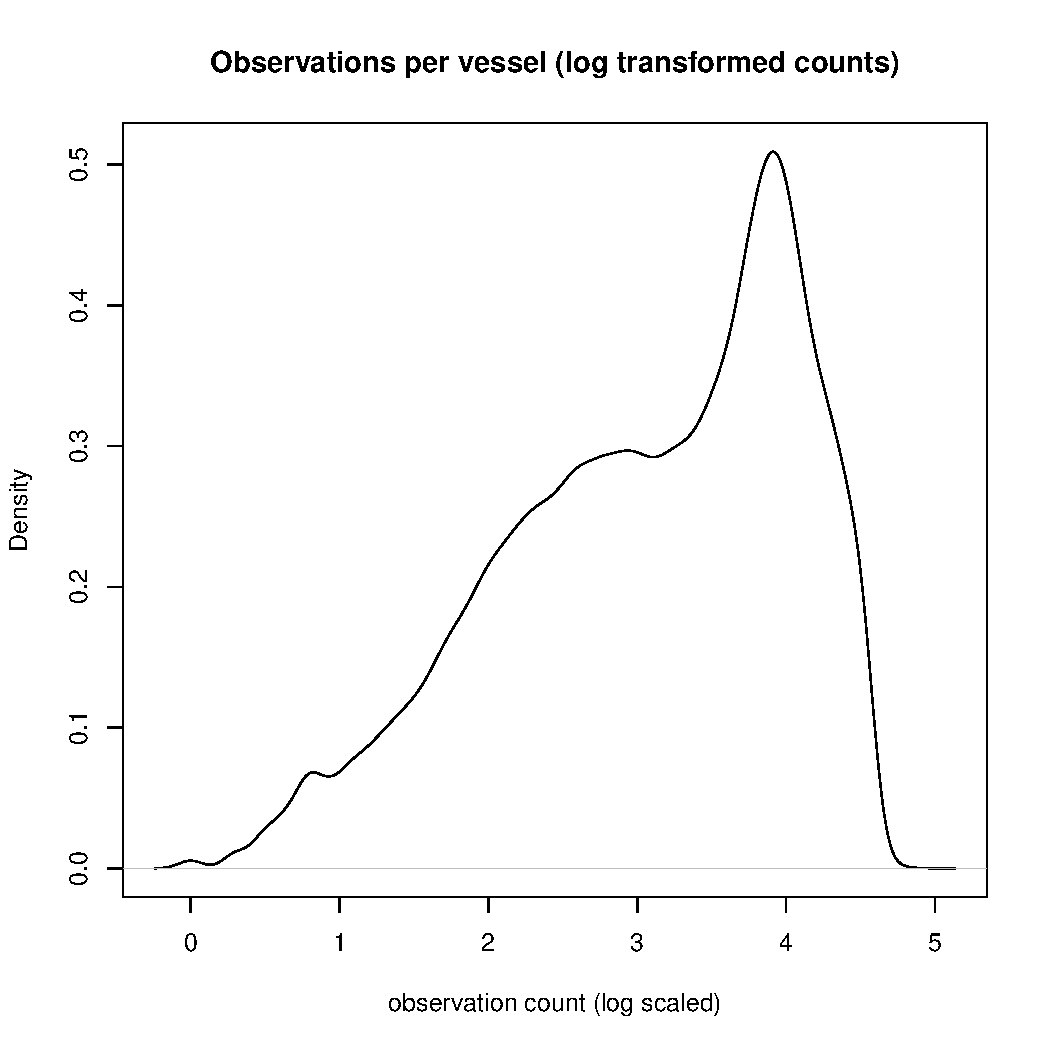
\includegraphics[width=100mm]{figures/obs-per-vessel-log.pdf}
  \caption{Number of observations per vessel, log scaled.}
  \label{fig:obs-per-vessel-log}
\end{figure}


% highlight importance of geometry + ATTRIBUTES. one alone is insufficient, both can be powerful.

%An aside on 'ships' - ships can have multiple callsigns, MMSI idenfiers, and other data which ideally would locate a specific vessel. We handle this ambiguity methods -- a full version of this can go into supplementals, but worth covering here, because we can map \textbf{type} from observed behavior -- fishing vs. cargo vs. cruise is all obvious when looking at the movement patterns (fold into above 'filtering process' section)

Another important point is that while ship attributes provide us some details as to their nature, categories (such as tanker or cargo) are not based purely on attributes, but also include movement patterns. This is a distinguishing characteristic between the data, as different classes of vessel show distinct movement patterns, which is useful both in validation, and as an output product, since vessel classes have differing effects and interactions. Because this data is stored in a spatial database, I link derived representation back to the records that formed it. While this is a common feature of spatial databases, it is an important trait since data are often provided as simple 'end products' without the provenance to understand its limitations.

% XXX above is good, expand it

%Can link data representations all the way back to attributes of raw data [note: this is true in many spatial databases, right? what makes it special here?]
% - often a requirement but only get 'end products' instead without detailed attributes, or conversely all details on one ship but no way to move between realms fluidly.

\subsection{Data Representations}

% It is necessary to have multiple representations of the data - the data model must flow from the question asked (goodchild, also anything in ebook on GISci?)

After filtering and validating the data as described, I build data representations which bring us closer to answering some of the problems raised in the introduction. Frequently there is no single optimal representation of data, but instead a set of representations which, when matched to particular uses, can be combined to provide insight.

Here, I look at how maintaining both discrete object and continuous fields representations (Figure \ref{fig:representation-in-gis}) allows us to address questions about shipping, including its ecological effects. While the point data alone is too simple for making predictions related to these phenomena, incorporating too much complexity risks making computation infeasible~\citep{de2007geospatial}.

% Some of the effects. link up how specific effects could be monitored by our different representations. Can't just use points to predict phenomena of this nature, but can't incorporate full complexity of reality either; chosen representations are a compromise between those two extremes.

% As in \ref{fig:representation-in-gis}, we can keep track of the ships in a discrete object representation, and after filtering the observations, converting the individual ship locations into movement tracks.

% Merger of data - which can give a single representation of the data

\begin{figure}[htbp]
  \centering
  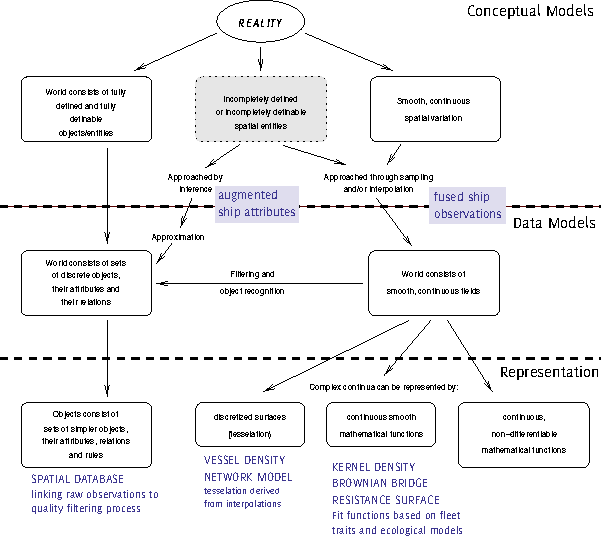
\includegraphics[width=160mm]{figures/representation-in-gis.pdf}
  \caption{GIS abstractions, this work's specific {\color{DBlue} additions in blue}. Adopted from \cite{Bivand2011}}
  \label{fig:representation-in-gis}
\end{figure}

% It is necessary to have multiple representations of the data - the data model must flow from the question asked (goodchild, also anything in ebook on GISci?)

%Want to link representation to USE, lack of a single simple view which meets all needs. counterpoint to the 'single metric' perspective. 
% [have note: 'link to stats', but now unsure what that means].

% Store the raw observations in a spatial database (PostGIS), use parallelized code to quickly aggregate the results.
\subsection{Ship Types}

% XXX open problem: what designates a 'ship'?
%   Hal: `The biggest flaw is that, long ago, I assumed one ship == one callsign. It turns out, of course, that a single ship can have multiple callsigns (due to sale or reflagging), and that a single callsign can be assigned to multiple ships (e.g. NOAA, and also the Queen Mary/Queen Mary II). So the db really needs its own internal ship UID.`

%  Hal, on 'using MMSI + IMO + Callsign'--  Yeah, that still misses reflagging. I think what I will end up with is a "find-or-create ship with IMO,MMSI,Callsign", together with a manual process for me to force the database to combine two different ship UUID's that actually refer to the same ship. Even that isn't enough, because we see misprogrammed AIS units with dummy MMSI's, and fleetwide MMSI's."

%    ... Almost want a probabilistic model of what ship it is based on the information we do have reliably, and cross-validation with the various online databases... perhaps even validation with Equasis? Could do this for a small subset of the ships, but clearly not them all.

% XXX   - create a ship 'UUID' like feature which incorporates the different aspects: IMO, MMSI, Callsign, Name... we care about specific _ships_ not necessarily what line they're running under or other changes, though this is useful information for certain classes of questions.

%  - collapse all redundant columns from the database once we have this hybrid observation model and can safely assign individual records to a particular ship (instead of a guess based on say, MMSI, which may be misprogrammed).

% XXX mention the ontology work in this space: there are people thinking about this stuff, but it isn't where we need it to be.
% \cite{Vries2009}
% IALA Guideline No. 1028 On The Automatic Identification System (AIS)

An open problem within the maritime community is: what designates a ship? Ships can be classified on a variety of dimensions, including propulsion form, hull material, function and many others. Ontologies have been in development to solve this problem \citep{Vries2009}, but here I focus on use: what is the primary activity the vessel is engaged in? Starting with the initial classes provided by our data sources, I collapsed them into nine major functional groups (Table \ref{table:ships-by-type}). Because the full attributes of each vessel are retained, and frequently include multiple type labels, it is possible to break this down further for future analyses, but these broad classes served well for classifying distinct movement patterns.

Identifiers -- what ship is this -- similarly poses a problem. By incorporating information from many different identifiers and focusing on those less changeable, such as IMO number and radio callsign, we increase the chances of valid matches. But additional attributes such as the Maritime Mobile Service Identity (MMSI), and vessel name are often equally useful, particularly because they are broadcast alongside each AIS record. Vessel operators may fail to maintain this information, so it becomes important to cross validate the attributes to gain reasonable match rates.

% SHIP CLASSES! HOW ARE THEY DEFINED, WHAT ARE THE DIMENSIONS BEING COLLAPSED?
%  a bunch of ways to classify (included in wikipedia article, I also have some notes we defined these by functional groups and their expected ecological differences

% overview of summary statistics of data
\begin{table}[htbp]
  \begin{tabular}{rrrrrr} %{\centering\arraybackslash}p{2cm}>{\centering\arraybackslash}p{5cm}>{\centering\arraybackslash}p{9cm}}
    \hline
    Type & Vessels \textit{(AIS)} & Vessels \textit{(VOS)} & fleet size & coverage (\%) & observations (M) \\
    \hline
    Cargo & 25214 & 5838 & 33392\textsuperscript{1} & 75.6 & 665.45 \\
    Tanker & 9758 & 2375 & 14068\textsuperscript{1} & 69.4 & 264.42 \\
    Passenger & 4007 & 777 & 6370\textsuperscript{1} & 62.9 & 142.16 \\
    Support & 9954 & 735 & 25234\textsuperscript{1} & 39.4 & 298.02 \\
    High-speed & 404 & 81 & 1178 & 34.3 & 2.52 \\
    Fishing & 11186 & 349 & 51200\textsuperscript{3} & 21.8 & 6.87 \\
    Pleasure & 20727 & 661 & 800,000\textsuperscript{2} & 2.59 & 267.48 \\
    Other & 9507 & 1400 & -- & -- & 4.75 \\
    Authority & 656 & 55 & -- & -- & 1.44 \\
  \end{tabular}
  \caption{Summary of analyzed ship data\\
  1. \cite{Equasis2011}.\\
  2. \cite{westwood2001global}.\\
  3. \cite{FAOfishing}.}
  \label{table:ships-by-type}
\end{table}
% XXX: high-speed craft from ISL? can't find original ref
% NOTE: the FAO estimates the _full_ fishing fleet size at 4 million vessels, the size clearly has an important effect.
% see: fleet-size.txt for details on this table.


\subsubsection{Raw point data}

% \begin{itemize}
%   \item geoatom with time $\langle x,t,z \rangle$
%   \item formalize what these observations mean
%   \item apply filtering using space-time + attributes
% \end{itemize}

Records are sampled at 600 second intervals (10 minutes). For most ship classes, this sample rate retains the movement patterns, and is a similar sample rate to studies using aggregation to remove noise, like \citep{Vries2009}, which uses piecewise aggregate approximation with w = 30 (300 seconds) to ``strike a good balance between capturing the general movement and ignoring noise''. % XXX NOTE: this is a filtering technique, so it isn't a direct mapping onto the reduced fidelity data we're using.

The spatial databases' historical focus was on accuracy \citep{goodchild1989accuracy}. This showed the value in retaining raw observations, both by minimizing lossy transformations, and providing multiple models of the same data to retain consistency with reality.

\subsubsection{Tracks}

Tracks convert discretely sampled time points into a interpolated continuous phenomena. The uncertainty surrounding the interpolation can be described by a time prism (Figure \ref{fig:time-prism}), which bounds the area based on the maximum velocity of the object at motion. Here, I first constrain the track segments to have movement above 0.5 Kt/hr, below which vessel control is difficult, and an upper bound of 40 Kt/hr, derived empirically from our ship speed distributions (See Figure \ref{fig:vessel-speed-density}). Next I require observations have coordinates bounded by the coordinate space, and exclude any beyond the surface of the earth. I further require that to be considered a track, the above criteria must be met for at least one segment of that vessels transit. The ships are then constrained to move along the shortest distance on a geoid, or great circles, using GeographicLib \citep{karney2012algorithms}. This information is reused in computing the speed along each segment.
% pulled from tracks/shipping_tracks_obs_validated.py

\begin{figure}[h!]
  \centering
    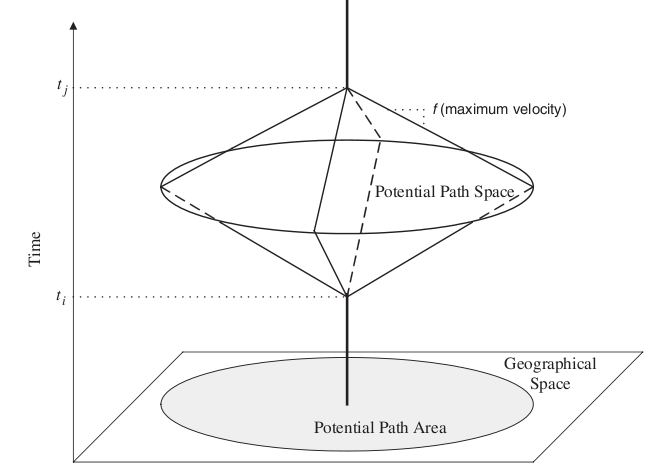
\includegraphics[width=80mm]{images/measurement-theory-for-time-geography-prism.png}
  \caption {A simple space{\textendash}time prism, as in \citep{Miller2005}; original from \citep{Wu2002}}
  \label{fig:time-prism}
\end{figure}

%   \item link to time geography... Hagerstrands conceptual framework... Literature on T-GIS as tracking.
%   \item Goodchild lecture on T-GIS mentioned track interpolation, inferences about activity, track convergence, etc
 % [perhaps drop this for the time being... don't have lit built up on it, unless we can use the anomaly detection stuff]

\subsubsection{Field-based models}

Initially, kernel density estimation was used to produce field based estimates. However, based on the data volume, it proved more useful to provide models directly from discretized tracks, which are used in the two following datasets.

\paragraph{Ship density by type}

The primary output of this work is a field-based density model of ship movement. This view is useful in a wide variety of contexts, from extercises in marine spatial planning (MSP) to detecting conflict zones between resource users, and the simple density estimation in \cite{Halpern2008} remains a highly requested product. % XXX provide better examples
% XXX Why this matters: the view most people want to see; counts of X where and when. Useful for MSP, conflict resolution, detecting conflict zones, etc

Each vessel track was rasterized to both an 90 arcsecond grid (\textasciitilde{}5.5km at the equator) and an equal area grid in the Hobo Dyer projection (Figure \ref{fig:eu-cargo-density}). The latter case insures that the density function is computed on grid cells representing the same area for each cell, unlike the geographic grid where area varies by latitude. A vessel is counted only once for each cell it passes through, as the focus here os on overall movement patterns, and this criteria helps de-emphasize vessels with limited movement. Each raster vessel track was combined using simple map algebra to produce density maps for both the AIS and VOS data, for each of our vessel classes.

For each cell the output density value s calculated as a standardized equal-weighted addition between the two input datasets, AIS and VOS:
\begin{equation}
 s = \frac{R_{AIS}}{max(R_{AIS})} + \frac{R_{VOS}}{max(R_{VOS})} 
\end{equation}

\begin{figure}[h!]
  \centering
    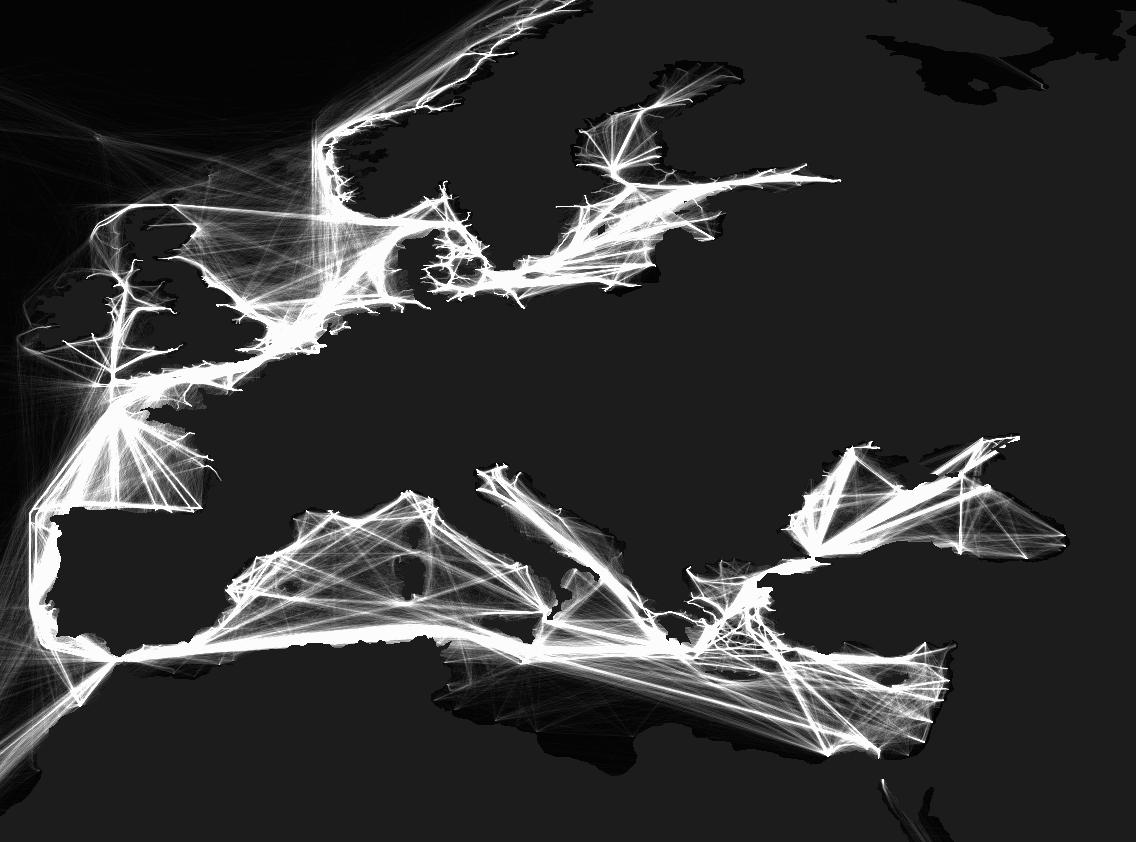
\includegraphics[width=120mm]{figures/cargo-lanes-eu-cropped.png}
  \caption {Cargo density grid, generated by combining AIS and VOS records.}
  \label{fig:eu-cargo-density}
\end{figure}

% Bresenham's line algorithm used for rasterizing the tracks. Only counted a ship moving through a single cell once to get movement patterns v. dockage

\paragraph{Speed density estimations of ships by ship type}

Ship speed plays a critical role in determining the survivability of collisions for many marine species~\citep{Vanderlaan2009}. Speed also directly relates to the emissions profile of a vessel, and it has been shown that speed reduction alone can reduce 50-80\% of greenhouse gas emissions \cite{lack2011impact}. Conversely, decreased speeds require more vessels to ship the same volume of goods or passengers, though companies such as Maersk are mitigating this by moving to significantly larger container ships.

Average speed per cell was calculated as sum speed over all observations $R_{AIS} \cup R_{VOS} = n$, and dividing it by the total number of observations, but only for those locations where a sufficient density $s$ is present: 

\begin{equation}
 \bar{s} = \left\{
   \begin{array}{l l}
    \frac{\sum\limits_{i=0}^n s}{x} & \quad \text{$s \ge 10$}\\
    0 & \quad \text {$s < 10$}
   \end{array}\right.
\end{equation}

% CLARIFY: what are the other effects of speed? anomaly detection?

% calculated the ship average speed over the journey, used that as 'speed value' [pretty bogus, but was quick and I couldn't get the M values in OGR correctly].
% XXX ADD THIS BACK? probably a new paper at that point.
%\subsubsection{Network model of ship travel}

%Some analyses require 'factoring out' geography to the extent possible, such as ecological models (Tilman book), Economic, et cetera. Network theory provides a useful basis of analysing geographically explicit data in a mathematical framework which can incorporate some of the geographic constraints while eliding many details necessary in a spatially-explicit model.

%Best thing here is Kaluza but they totally lost the geography in transit -- can produce a middle ground model which has geographic nodes and edges, but still retains the rigour of the network model. Can get both!

% ...

% Paragraph from one of my position papers --
% One model I’m particularly interested in is hybridized network models using tools like NetworkX, which have the attractive property of allowing mixed field/object representations of the same data simultaneously, hence escaping the common limits of networks as mentioned in ? of every link or edge requiring a discrete value. By imbuing a network model with object-oriented features, some of the challenges I’ve been having representing my ship traffic data vanish. An- other advantage of manipulating graphs as a primitive is their widespread support, including general purpose graph databases which are particularly taking off in the semantic space.

% another pp from a position
% This becomes particular important as the tools of spatial thinking extend across disciplinary boundaries, both in the social and physical sciences (Goodchild and Janelle, 2010; Tilman and Kareiva, 1997). Other domains, such as ecology and economics, are coming to terms with the fact that their historical approaches to keeping simple models (and by extension, limiting model scope to their domain) ignores important spatial context which naturally arises at the unit of analysis (Tilman and Kareiva, 1997; Krugman, 1991).

\subsection{Record Linkage}

By combining authoritative data from a variety of sources (Table \ref{table:ships-data-sources}), we can reconcile our observations, greatly improving the quality of resulting ship movement models. Though we do include two authoritative datasets, the sources are inconsistent, and require an initial step of cross-linking records. This approach was initially developed with medical records, and more recently developed as the record linkage field in computer science~\citep{Christen2012}.

% table describing sources
% SOURCES: ship-id-model.txt
%          ship-id-model/linkages.txt
\begin{table}[htbp]
  \begin{tabular}{rrrrl}%{\centering\arraybackslash}p{2cm}>{\centering\arraybackslash}p{5cm}>{\centering\arraybackslash}p{9cm}}
    \hline
    Source & Code & Records & Cross-linked & Attributes \\
    \hline
     Digital Seas & DS & 212166 & 68002 & {\footnotesize name, IMO, MMSI, callsign, type, width, length} \\
      FCC\textsuperscript{1} ULS\textsuperscript{2} & FCC & 319964 & 24531 & {\footnotesize name, MMSI, callsign, class, gross gonnage, length} \\
      ITU\textsuperscript{3} MARS\textsuperscript{4} & ITU & 372183 & 75928 & {\footnotesize name, IMO, MMSI, callsign, class, owner, gross tonnage}\\ 
     VesselTracker & VT & 126534 & 83372 & {\footnotesize name, IMO, MMSI, callsign, class, length}
  \end{tabular}
  \caption{Ship data sources.\\ 
  1. Federal Communications Commission \\ 
  2. Universal Licensing System \\
  3. International Telecommunication Union \\ 
  4. Maritime mobile Access and Retrieval System}
  \label{table:ships-data-sources}
\end{table}

I built a probabilistic model which evaluated all possible pairwise combinations between source records. By using the methodology of record linkage, a set of rules was developed to map records between the six possible source pairs. Each pair was evaluated for common, consistent attributes, and compared against these columns. The software package used, (FRIL, \citealp{Jurczyk2008fril}), provides an Expectation Maximization algorithm to iteratively optimize the column weighting, but due to the large number of records, this proved ineffective. Instead, samples were examined, and the criteria were set by manual tuning both the weightings and acceptance levels to match a training dataset of valid linkages (Table \ref{table:ships-record-linkage-methods}). 

% table describing the record linkage technique used for each data source
% SOURCE: record-linkage/FRIL/config/*.xml
\begin{table}[htbp]
  \begin{tabular}{rrrrrr} %{\centering\arraybackslash}p{2cm}>{\centering\arraybackslash}p{5cm}>{\centering\arraybackslash}p{9cm}}
    \hline
    Source $A$ & Source $B$ & acceptance level & column & distance metric & weight \\
    \hline
     DS & ITU & 92 & callsign & Jaro-Winkler\textsuperscript{1} & 50 \\
        &     &    & MMSI & equal & 40 \\
        &     &    & name & Jaro-Winkler & 40 \\
     DS &  VT & 85 & callsign & Jaro-Winkler & 60 \\
        &     &    & IMO & Jaro-Winkler & 20 \\
        &     &    & name & Jaro-Winkler & 20 \\
    FCC & ITU & 85 & callsign & Jaro-Winkler & 95 \\
        &     &    & name & Jaro-Winkler & 5 \\
    FCC &  VT & 95 & callsign & Jaro-Winkler & 66 \\
        &     &    & name & Jaro-Winkler & 5 \\
        &     &    & MMSI & Jaro-Winkler & 24 \\
        &     &    & length & equal & 5 \\
     VT & ITU & 80 & callsign & Jaro-Winkler & 20 \\
        &     &    & MMSI & Edit Distance & 30 \\
        &     &    & name & Jaro-Winkler & 10 \\
        &     &    & IMO & Jaro-Winkler & 40 \\
     DS & FCC & 95 & callsign & equal & 99 \\
        &     &    & name & Jaro-Winkler& 1 \\
  \end{tabular}
  \caption{Ship record linkage methods used. \\
    \textsuperscript{1} Jaro-Winkler distance \citep{winkler1990string}: length $l = 4$ and scaling factor $p = 0.1$}
  \label{table:ships-record-linkage-methods}
\end{table}


For most attributes, either the equal fields (both values are the same) or the Jaro-Winkler distance metric were used. Jaro-Winkler has useful properties for this data: it is effective on both numeric and textual data, and is particularly good in picking up the kinds of errors inherent in user provided data sources such as those used in this study. A study of string comparison metrics found it to be both efficient, and effective, with a high match rate on diverse data~\citep{Cohen2003}. The equations used in the Jaro-Winker distance are described in (Appendix \ref{sec:record-linkage-appendix}).

Once each combination between two sources was finished running in FRIL, a second rule-based method was developed to capture valid pairings initially missed. If vessels had equality in any two attributes of the set ${MMSI, callsign, name}$, if callsign and vessel length matched, or if the IMO number provided was a valid seven digit number, then the pair was marked as linked. This was tested against a number of pairs manually, and successfully caught many of the initially missing yet valid linkages.

\subsubsection{Linkage Validation}

After pairwise linkage, matched records (Table \ref{table:ships-record-linkage-results-summary}) were further cross-linked, % XXX HOW? create-ships-table.py contains the logic.
 to account for vessels appearing in multiple sources. The number of links per ship averaged 3.5 ($\mu = 3.49, \sigma = 0.828$), % XXX STATISTICALLY SIGNIFICANT? the vast majority only have 3-4 links. Tried fitting this data to a variety of distributions, it can be done, but for what end? the 'high' values really indicate errors, and these should be separated out to their relevant subships.
though this distribution is skewed by a handful of vessels which were linked to many vessels incorrectly. To correct these problems and measure the effectiveness of the record linkage steps, I performed validation using the techniques which follow.

Detecting errors in this data is particularly problematic, as the records are highly correlated by nature -- often, IMO number, callsign and name differ by only one character for two ships in the same fleet. We want to keep these kinds of vessels separate, while simultaneously finding small differences due to entry error, which proved difficult. I developed a validation score to remove over-aggressive links between the data, and allow us a second quality check which is tunable to threshold the data, depending on the kinds of error we are willing to accept.

To start with, I evaluated the bad joins present in the data, and the specific traits that were common across the sample. These included:
\begin{enumerate}[noitemsep]
 \item >6 linked records
 \item >1 radio callsign
 \item >1 MMSI
 \item clear name mismatches
 \item vessel assigned to multiple incompatible classes
\end{enumerate}

Based on this, a set of rules was developed to assign a validation score and probable vessel class based on the inputs.  Again Jaro-Winkler was used to compare attribute matches for both ship name and radio callsign, with $1 - d_w$ being added to the validation score. For attributes that had a single value, the attribute score was increased by one, otherwise vessels which had more than two MMSIs or five linked records had one point removed from their validation score. Lastly, if a ship was identified as being in multiple incompatible classes, one point was subtracted for each additional class. Our final scores for all vessels is shown in (Figure \ref{fig:validation-score-hist}).

\begin{figure}[h!]
  \centering
    \includegraphics[width=90mm]{figures/validation-scores-hist.pdf}
  \caption {Validation scores, bin width=0.3}
  \label{fig:validation-score-hist}
\end{figure}

These scores were then used to select valid vessels, and to assign vessels to the nine classes. Only scores exceeding zero were used for the movement models. Finally, though all these steps give us good self-consistency, I wanted to test against even better sources.  % TODO: perform data validation on these observations with Equasis. Sample a handful of records from each class, then perform the validation.
While some of our input datasets are authoritative, the best available data remains commercial. A a 1\% sample of the records were compared to those provided in Equasis \citep{Equasis2011}, which includes validated records from the commercial fleet. This showed that, after cross-linking, the validation score showed good correpsondence with true vessels, though only comparisons to commercial classes of vessels were possible.

% XXX built spatial indexes and reordered the data on disk to match for performance.
